\documentclass[landscape,final]{baposter}

\usepackage[utf8]{inputenc}

\usepackage{times}
\usepackage{calc}
\usepackage{graphicx}
\usepackage{amsmath}
\usepackage{amssymb}
\usepackage{relsize}
\usepackage{multirow}
\usepackage{bm}
\usepackage{array}
\usepackage{bibspacing}

\usepackage{graphicx,capt-of}
\usepackage{multicol}

% \usepackage{pgfbaselayers}
\pgfdeclarelayer{background}
\pgfdeclarelayer{foreground}
\pgfsetlayers{background,main,foreground}

\usepackage{helvet}
%\usepackage{bookman}
\usepackage{palatino}

\renewcommand{\refname}{}
\def \figdir {../figures}

\newcommand{\captionfont}{\footnotesize}

\selectcolormodel{cmyk}

\graphicspath{{images/}}

%%%%%%%%%%%%%%%%%%%%%%%%%%%%%%%%%%%%%%%%%%%%%%%%%%%%%%%%%%%%%%%%%%%%%%%%%%%%%%%%
%%%% Some math symbols used in the text
%%%%%%%%%%%%%%%%%%%%%%%%%%%%%%%%%%%%%%%%%%%%%%%%%%%%%%%%%%%%%%%%%%%%%%%%%%%%%%%%
% Format
\newcommand{\Matrix}[1]{\begin{bmatrix} #1 \end{bmatrix}}
\newcommand{\Vector}[1]{\Matrix{#1}}
\newcommand*{\SET}[1]  {\ensuremath{\mathcal{#1}}}
\newcommand*{\MAT}[1]  {\ensuremath{\mathbf{#1}}}
\newcommand*{\VEC}[1]  {\ensuremath{\bm{#1}}}
\newcommand*{\CONST}[1]{\ensuremath{\mathit{#1}}}
\newcommand*{\norm}[1]{\mathopen\| #1 \mathclose\|}% use instead of $\|x\|$
\newcommand*{\abs}[1]{\mathopen| #1 \mathclose|}% use instead of $\|x\|$
\newcommand*{\absLR}[1]{\left| #1 \right|}% use instead of $\|x\|$

\def\norm#1{\mathopen\| #1 \mathclose\|}% use instead of $\|x\|$
\newcommand{\normLR}[1]{\left\| #1 \right\|}% use instead of $\|x\|$

%%%%%%%%%%%%%%%%%%%%%%%%%%%%%%%%%%%%%%%%%%%%%%%%%%%%%%%%%%%%%%%%%%%%%%%%%%%%%%%%
% Multicol Settings
%%%%%%%%%%%%%%%%%%%%%%%%%%%%%%%%%%%%%%%%%%%%%%%%%%%%%%%%%%%%%%%%%%%%%%%%%%%%%%%%
\setlength{\columnsep}{0.7em}
\setlength{\columnseprule}{0mm}


%%%%%%%%%%%%%%%%%%%%%%%%%%%%%%%%%%%%%%%%%%%%%%%%%%%%%%%%%%%%%%%%%%%%%%%%%%%%%%%%
% Save space in lists. Use this after the opening of the list
%%%%%%%%%%%%%%%%%%%%%%%%%%%%%%%%%%%%%%%%%%%%%%%%%%%%%%%%%%%%%%%%%%%%%%%%%%%%%%%%
\newcommand{\compresslist}{%
\setlength{\itemsep}{1pt}%
\setlength{\parskip}{0pt}%
\setlength{\parsep}{2pt}%
}

%%%%%%%%%%%%%%%%%%%%%%%%%%%%%%%%%%%%%%%%%%%%%%%%%%%%%%%%%%%%%%%%%%%%%%%%%%%%%%
%%% Begin of Document
%%%%%%%%%%%%%%%%%%%%%%%%%%%%%%%%%%%%%%%%%%%%%%%%%%%%%%%%%%%%%%%%%%%%%%%%%%%%%%
% \renewenvironment{list}{\begin{list}}{\end{list}}
\newenvironment{llist}{\begin{list}{$\bullet$}{\leftmargin=1em \itemindent=0em \parskip=0em \parsep=0pt}}{\end{list}}
\begin{document}
\setlength{\bibspacing}{\baselineskip}



%%%%%%%%%%%%%%%%%%%%%%%%%%%%%%%%%%%%%%%%%%%%%%%%%%%%%%%%%%%%%%%%%%%%%%%%%%%%%%
%%% Here starts the poster
%%%---------------------------------------------------------------------------
%%% Format it to your taste with the options
%%%%%%%%%%%%%%%%%%%%%%%%%%%%%%%%%%%%%%%%%%%%%%%%%%%%%%%%%%%%%%%%%%%%%%%%%%%%%%
\typeout{Poster Starts}
\background{
  \begin{tikzpicture}[remember picture,overlay]%
    \draw (current page.north west)+(-2em,-0em) node[anchor=north west] {\hspace{-2em}\includegraphics[height=1.1\textheight]{silhouettes_background}};
  \end{tikzpicture}%
}
\definecolor{skyblue}{rgb}{0.87,0.9,1}
\definecolor{white}{rgb}{1,1,1}
\definecolor{black}{cmyk}{0,0,0.0,1.0}
\definecolor{darkYellow}{cmyk}{0,0,1.0,0.5}
\definecolor{darkSilver}{cmyk}{0,0,0,0.1}
\definecolor{darkblue}{rgb}{0,0,0.7}
\definecolor{lighterryellow}{cmyk}{0,0,0.2,0.0}
\definecolor{lightyellow}{cmyk}{0,0,0.3,0.0}
\definecolor{lighteryellow}{cmyk}{0,0,0.1,0.0}
\definecolor{lightestyellow}{cmyk}{0,0,0.05,0.0}
\begin{poster}{
  % Show grid to help with alignment
  grid=no,
  % Column spacing
  colspacing=1em,
  % Color style
  bgColorOne=white,
  bgColorTwo=white,
  borderColor=blue,
  headerColorOne=skyblue,
  headerColorTwo=black,
  headerFontColor=black,
  boxColorOne=white,
  boxColorTwo=skyblue,
  % Format of textbox
  textborder=rounded,
  % Format of text header
  eyecatcher=yes,
  headerborder=open,
  headerheight=0.12\textheight,
  headershape=rounded,
  headershade=plain,
  headerfont=\Large\textsf, %Sans Serif
  boxshade=plain,
%  background=shade-tb,
  background=plain,
  linewidth=2pt
  }
  % Eye Catcher
  {
\includegraphics[height=6em]{figures/Bogazici_University_Logo.png}} % No eye catcher for this poster. If an eye catcher is present, the title is centered between eye-catcher and logo.
  % Title
  {\sf \vspace{5pt}%Sans Serif
  %\bf% Serif
  \vspace{-14pt}
  LDA Based Similarity Modeling for Question Answering on a Turkish Wikipedia
}
  % Authors
  {\sf \Large \vspace{5pt} %Sans Serif
  	\textbf{İsmet Burak Kadron and Çağıl Uluşahin Sönmez}\\
    Department of Computer Engineering, Bo\u{g}azi\c{c}i University, Istanbul, Turkey\\
    \{ismet.kadron, cagil.ulusahin\}@boun.edu.tr

  }
  % University logo
  {
\includegraphics[height=7em]{figures/Bogazici_University_Logo.png}
  }

  \tikzstyle{light shaded}=[top color=baposterBGtwo!30!white,bottom color=baposterBGone!30!white,shading=axis,shading angle=30]

  % Width of left inset image
     \newlength{\leftimgwidth}
     \setlength{\leftimgwidth}{0.78em+8.0em}

%%%%%%%%%%%%%%%%%%%%%%%%%%%%%%%%%%%%%%%%%%%%%%%%%%%%%%%%%%%%%%%%%%%%%%%%%%%%%%
%%% Now define the boxes that make up the poster
%%%---------------------------------------------------------------------------
%%% Each box has a name and can be placed absolutely or relatively.
%%% The only inconvenience is that you can only specify a relative position
%%% towards an already declared box. So if you have a box attached to the
%%% bottom, one to the top and a third one which should be in between, you
%%% have to specify the top and bottom boxes before you specify the middle
%%% box.
%%%%%%%%%%%%%%%%%%%%%%%%%%%%%%%%%%%%%%%%%%%%%%%%%%%%%%%%%%%%%%%%%%%%%%%%%%%%%%
    %
    % A coloured circle useful as a bullet with an adjustably strong filling
    \newcommand{\colouredcircle}[1]{%
      \tikz{\useasboundingbox (-0.2em,-0.32em) rectangle(0.2em,0.32em); \draw[draw=black,fill=baposterBGone!80!black!#1!white,line width=0.03em] (0,0) circle(0.18em);}}

%%%%%%%%%%%%%%%%%%%%%%%%%%%%%%%%%%%%%%%%%%%%%%%%%%%%%%%%%%%%%%%%%%%%%%%%%%%%%%
  \headerbox{Abstract}{name=abstract,column=0,row=0}{
%%%%%%%%%%%%%%%%%%%%%%%%%%%%%%%%%%%%%%%%%%%%%%%%%%%%%%%%%%%%%%%%%%%%%%%%%%%%%%
\par We present a generative model for a Question Answering system applied to a Turkish corpora. The problem is “answering a natural language question using relevant documents”. Topic modeling using LDA (Latent Dirichlet Allocation) to rank the similarities between a question and different passages in the document is a known method to solve this kind of problem as shown in the recent work of Celikyilmaz et. al. Their approach is multilingual however a morphologically rich language like Turkish might benefit a lot from a model that is fine tailored for such languages. \\
\par We propose a model that can handle the sparsity in MRLs (Morphological Rich Languages) better when compared to the original model. This model also takes syntactic properties (stems, inflectional affixes) into account because in MRLs substantial grammatical information, i.e., information concerning the arrangement of words into syntactic units or cues to syntactic relations, is expressed at word level. In the end, we apply both models to a Turkish corpora and compare the results. \\

}
%%%%%%%%%%%%%%%%%%%%%%%%%%%%%%%%%%%%%%%%%%%%%%%%%%%%%%%%%%%%%%%%%%%%%%%%%%%%%%
  \headerbox{Motivation}{name=intro,column=0,below=abstract}{
%%%%%%%%%%%%%%%%%%%%%%%%%%%%%%%%%%%%%%%%%%%%%%%%%%%%%%%%%%%%%%%%%%%%%%%%%%%%%%
	\par Question Answering (QA) is the task of automatic retrieval of an answer given a question. \\

}

%%%%%%%%%%%%%%%%%%%%%%%%%%%%%%%%%%%%%%%%%%%%%%%%%%%%%%%%%%%%%%%%%%%%%%%%%%%%%%
  \headerbox{Original Model}{name=exp,column=1,span=1}{
%%%%%%%%%%%%%%%%%%%%%%%%%%%%%%%%%%%%%%%%%%%%%%%%%%%%%%%%%%%%%%%%%%%%%%%%%%%%%%
	\par A passage in retrieved documents (document collection) is represented as a mixture of fixed topics, with topic $z$ getting weight $\theta^(s)_z$ in passage $s$ and each topic is a distribution over a finite vocabulary of words, with word $w$ having a probability $\phi^(z)_w$ in topic $z$. Placing symmetric Dirichlet priors on $\theta^(s)$ and $\phi^(z)$, where $\alpha$ and $\beta$, the generative model is given by: \\

\begin{equation*}
  \label{eq:dists}
  \begin{aligned}
    w_i|z_i, \phi_{wi}^{(z_i)} & \sim Discrete(\phi^{(z_i)}), \quad i = 1, ..., W \\
    \phi{(z)}  & \sim  Dirichlet(\beta), \quad z = 1, ..., K \\
    z_i | \theta^{(s_i)} & \sim  Discrete(\theta^{(s_i)}), \quad i = 1, ..., W \\
    \theta^{(s)} & \sim  Dirichlet(\alpha), \quad s = 1, ..., S \\
  \end{aligned}
\end{equation*}

	\par S is the number of passages, K is the total number of topics, W is the total number of words in the document collection, and $s_i$ and $z_i$ are passage and topic of the $i$th word $w_i$, respectively. \\

	\par Our goal is to calculate the expected posterior probabilities of a word in a candidate passage given a topic and expected posterior probability of topic mixings of a given passage. \\

\begin{equation*}
  \label{eq:model}
    \hat{ \phi}_{wi}^{(z_i)} = \frac{n^{WK}_{w_{i}k}+ \beta}{\sum^W_{j=1}n^{WK}_{w_{j}k}+ W \beta} \quad \hat{\theta}^{(s)} \frac{n^{SK}_{sk} +\alpha}{\sum^K_{j=1}n^{SK}_{sj}+ K \alpha}
\end{equation*}

	\par For comparison metric, we have used TODO Burak\\


  }
%%%%%%%%%%%%%%%%%%%%%%%%%%%%%%%%%%%%%%%%%%%%%%%%%%%%%%%%%%%%%%%%%%%%%%%%%%%%%%
  \headerbox{Proposed Model}{name=proposed,column=2}{
%%%%%%%%%%%%%%%%%%%%%%%%%%%%%%%%%%%%%%%%%%%%%%%%%%%%%%%%%%%%%%%%%%%%%%%%%%%%%%
\par TODO Çağıl\\
\par In the proposed model, the words in passages are transformed to their stems by using two different methods.\\
\par First method is identifying and removing inflectional affixes. \\
\par Second method is taking first N characters of the word. \\

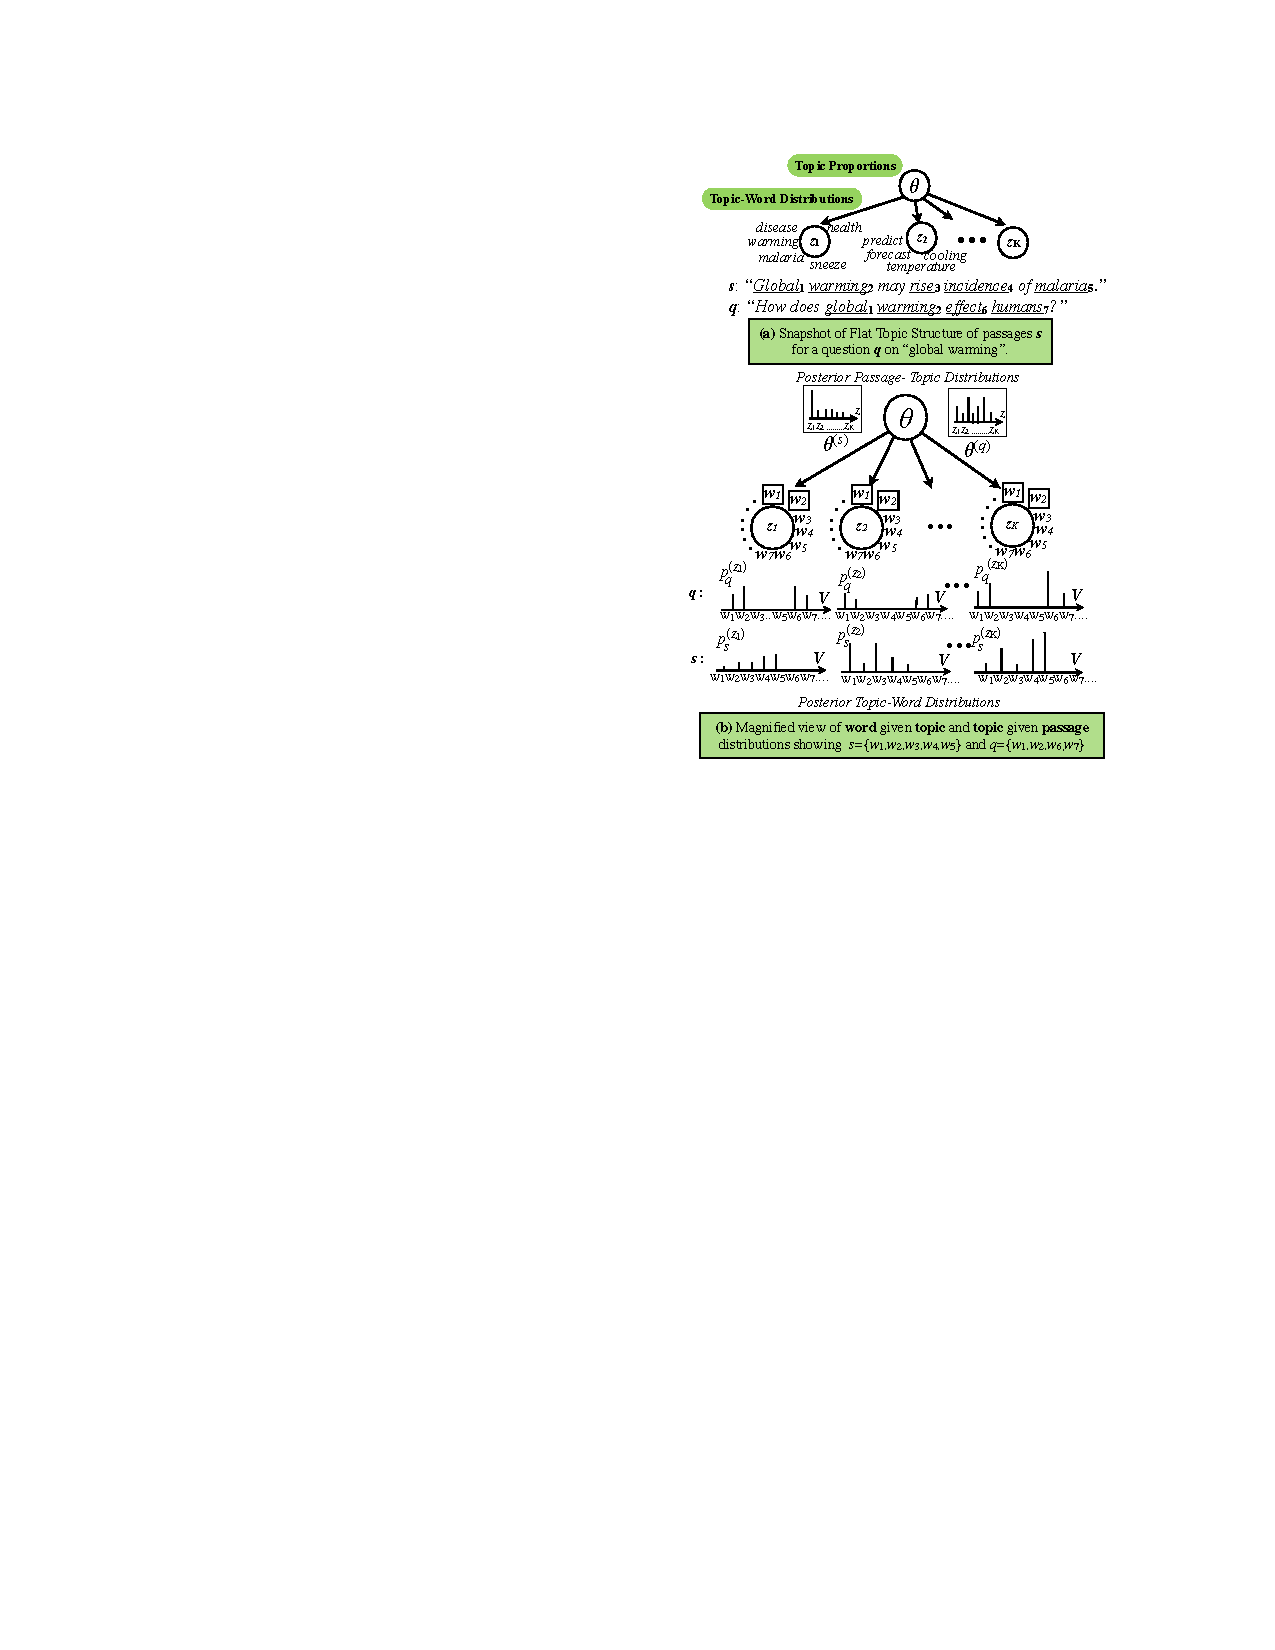
\includegraphics[scale=1.1]{./figures/model}
	\vspace{-12pt}
    \captionof{figure}{Topic-Word and Passage-Topic Distributions}
    \label{fig:figure}
\vspace{5pt}
}%

%%%%%%%%%%%%%%%%%%%%%%%%%%%%%%%%%%%%%%%%%%%%%%%%%%%%%%%%%%%%%%%%%%%%%%%%%%%%%%
\headerbox{Dataset and Results}{name=results,column=3,row=0}{
%%%%%%%%%%%%%%%%%%%%%%%%%%%%%%%%%%%%%%%%%%%%%%%%%%%%%%%%%%%%%%%%%%%%%%%%%%%%%%
\par We have used
}

%%%%%%%%%%%%%%%%%%%%%%%%%%%%%%%%%%%%%%%%%%%%%%%%%%%%%%%%%%%%%%%%%%%%%%%%%%%%%%
\headerbox{Acknowledgements}{name=ack,column=3,below=results}{
%%%%%%%%%%%%%%%%%%%%%%%%%%%%%%%%%%%%%%%%%%%%%%%%%%%%%%%%%%%%%%%%%%%%%%%%%%%%%%
\par We are grateful to Caner Derici and Yavuz Nuzumlalı for their help and support. We also want to thank Tunga Güngör and the team working with him on TÜBİTAK Project 113E036 for supplying us the data set and the opportunity to work further on their problem. \\
}

%%%%%%%%%%%%%%%%%%%%%%%%%%%%%%%%%%%%%%%%%%%%%%%%%%%%%%%%%%%%%%%%%%%%%%%%%%%%%%
  \headerbox{References}{name=references,column=3,below=ack}{
%%%%%%%%%%%%%%%%%%%%%%%%%%%%%%%%%%%%%%%%%%%%%%%%%%%%%%%%%%%%%%%%%%%%%%%%%%%%%%
\begin{tiny}
	\nocite{Spink2001731,Lind2005123,Cangar200853}
    \setlength{\parskip}{-2mm}
    \bibliographystyle{ieeetr}
    \bibliography{ref}
\end{tiny}
}%

\end{poster}%
%
\end{document}
